% !TEX root = ../Dokumentation.tex
\subsection{Beladen und Greifer}

\textbf{Funktionsbeschrieb}\\[0.2cm]
\begin{figure}[H]
\centering
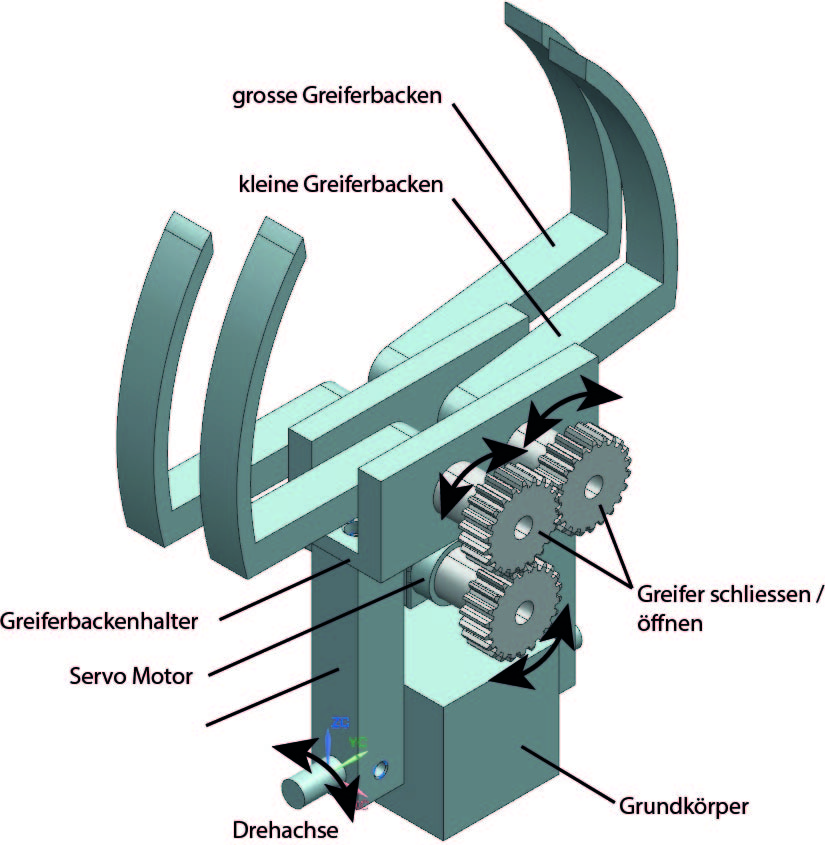
\includegraphics[width=0.5\textwidth]{03_Loesungskonzept/pictures/greifer3.jpg}
\caption{Greifer}
\end{figure}

Der Greifer ist auf der Grundplatte des Fahrzeuges montiert. Im Grundkörper wird die Welle für die Drehung des Greifers montiert. Die Welle wird von einem Servo Motor angetrieben. Um gute Laufeigenschaften zu erreichen werden Lagerbüchsen eingebaut. Auf der Drehachse sind die beiden Seitenplatten des Greifers montiert. Auf den Seitenplatten wird der Greifbackenhalter verschraubt.  Der Servo Motor für die Funktion Greifer schliessen/ öffnen wird am Greifbackenhalter befestigt. Auf dem Servo wird ein Zahnrad montiert, das über die gleichen Zahnräder die Greiferbacken öffnet/ schliesst. Die Greiferbacken sind so konzipiert, dass die 2 längeren und 2 kürzeren an verschiedenen Flächen greifen. Damit wird erreicht, dass der Container stabil bleibt während des ganzen Einladeprozesses. 

\begin{figure}[H]
\centering
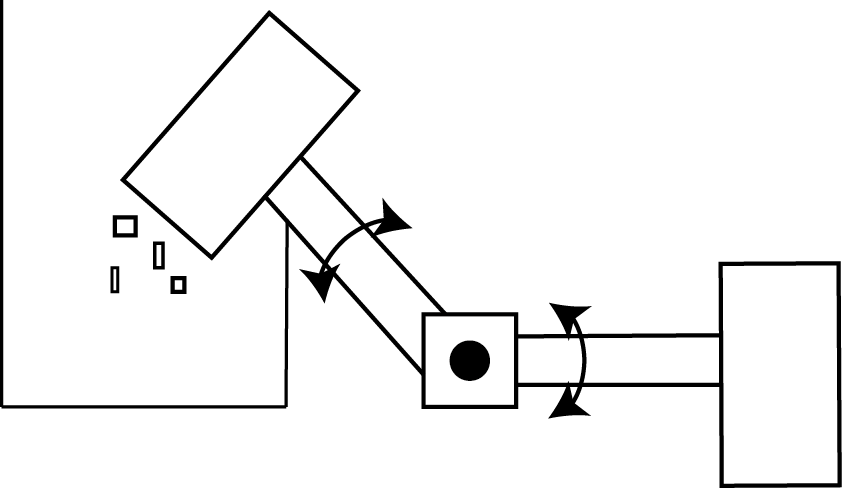
\includegraphics[width=0.5\textwidth]{03_Loesungskonzept/pictures/Beladen_1.png}
\caption{Einladeprozess}
\end{figure}

Der Greifer ist während des Fahren in oberer Position gelagert, damit die Abmasse der Aufgabenstellung eingehalten werden können. Der Greifer wird erst auf horizontale Richtung bewegt, nachdem der Wagen still steht und richtig positioniert ist.
Die rechte Fahrzeugkante wird auf 25mm +/- 5mm zum Trottoirrand positioniert. In Fahrtrichtung beträgt die maximale zulässige Positionierungenauigkeit +/- 10mm.

\begin{figure}[H]
\centering
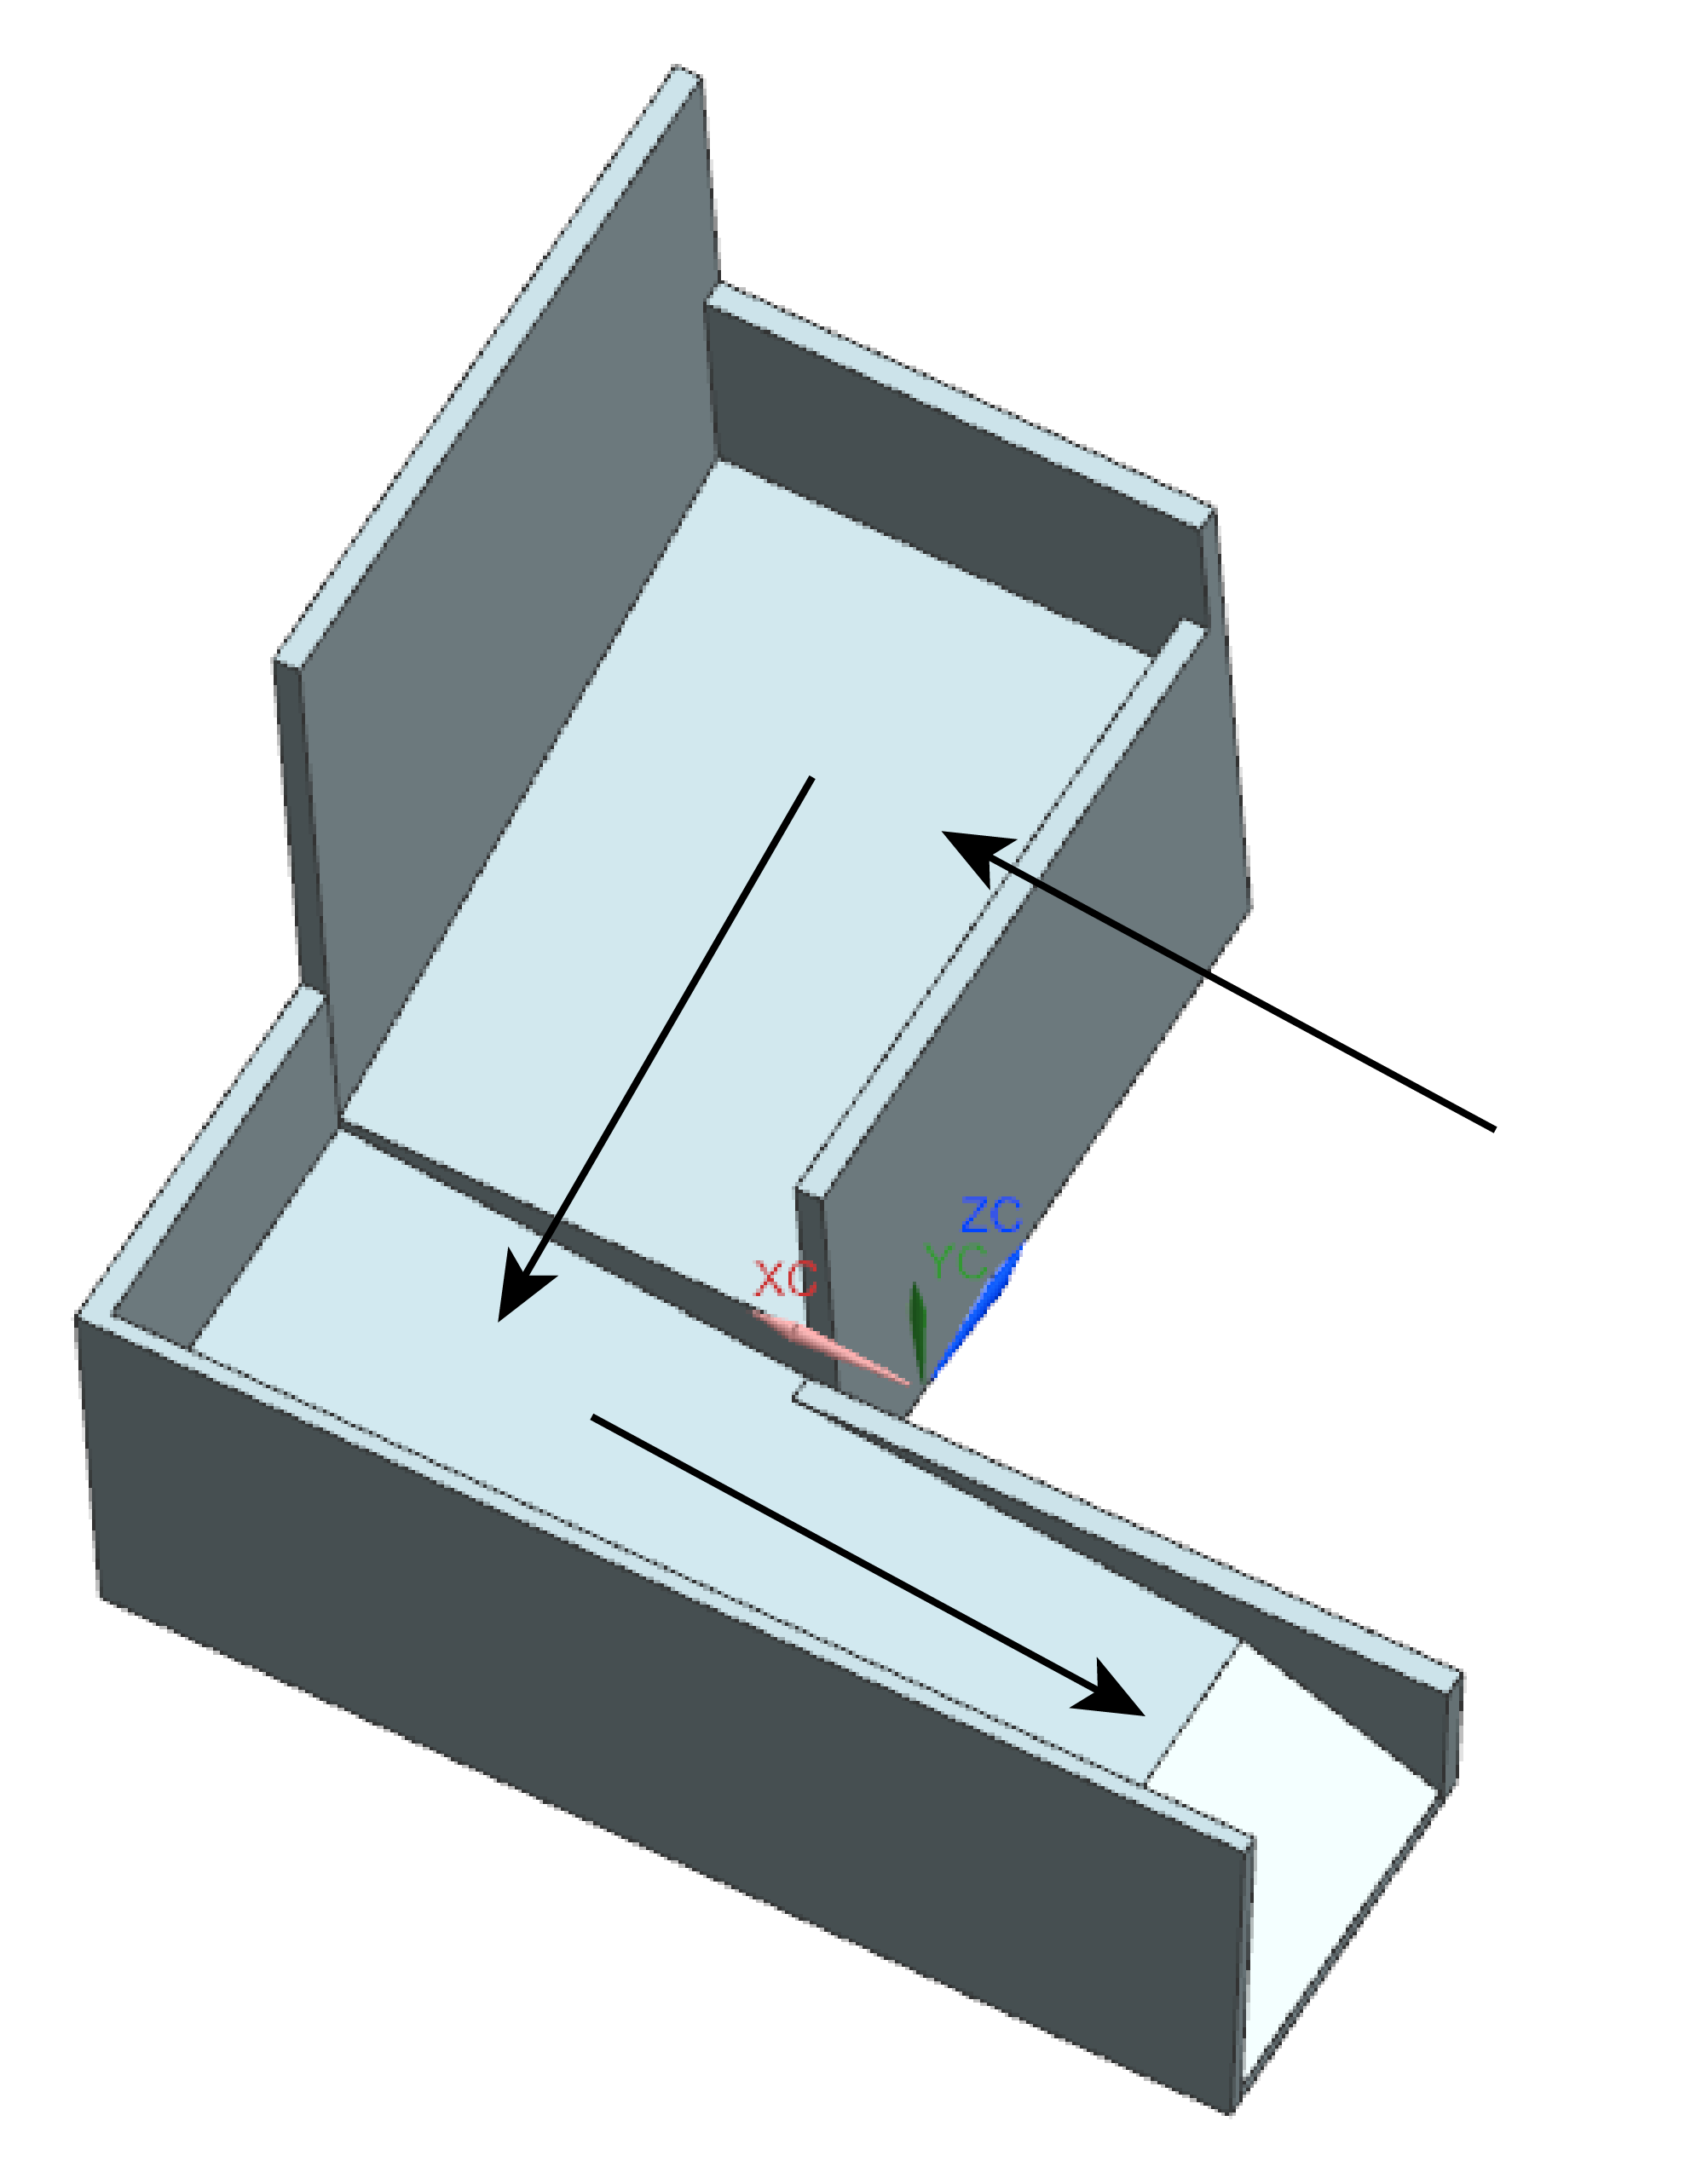
\includegraphics[width=0.5\textwidth]{03_Loesungskonzept/pictures/behaelter.png}
\caption{Schüttgutfluss in den beiden Behältern}
\end{figure}

Der Container wird in den ersten Behälter entleert. Durch den schrägen Boden fliesst das Schüttgut in den zweiten Behälter. Am Ende des zweiten Behälter wird ein Klappe montiert, damit die Schrauben und Mutter nicht herausfallen. Die Klappe wird durch einen Servo Motor gehalten und erst am Schluss beim Entladebehälter geöffnet.

\textbf{Komponentenbeschrieb}
\begin{itemize}
\item Zahnräder aus Kunststoff, Durchmesser = 15 (Einkaufteil)
\item Greiferbacken aus Kunststoff (Druckteil)
\item Grundkörper, Seitenplatte, Greifbackenhalter und Wellen werden aus Alu gefertigt.
\item Behälter aus Acrylglas 3mm Dicke (Laserzuschnitt)
\end{itemize}

Technische Daten der Motors Greifer:
\begin{itemize}
\item Stellzeit bei 4.8 Volt: 0.1 sec (50°) 
\item Stellzeit bei 6 Volt: 0.08 sec (50°) 
\item Betriebsspannung: 4.6/6 V
\item Stell-Moment bei 4.8 Volt: 18 Ncm
\item Stell-Moment bei 6 Volt: 20 Ncm 
\end{itemize}

Technische Daten des Motors Greifarm:
\begin{itemize}
\item Stellzeit bei 4.8 Volt: 0.19 sec (60°) 
\item Stellzeit bei 6 Volt: 0.17 sec (60°) 
\item Betriebsspannung: 4.6/6 V
\item Stell-Moment bei 4.8 Volt: 32 Ncm 
\item Stell-Moment bei 6 Volt: 35 Ncm 
\end{itemize}

\textbf{Berechnungen}
\\[0.2cm]
Servo Motor für Greifer schliessen /
Berechnung des benötigten Drehmoments: 
\begin{itemize}
\item Haftreibung auf 0.7 geschätzt
\item Masse Container m = 0.075kg
\item Gewichtskraft = m*g = 0.74 N
\item Kraft F = (0.5*0.74)/0.7 = 0.53 N
\item Abstand l = 80mm (Drehpunkt zu Greiffläche)
\item M = F*l = 0.04 Nm = 4 Ncm
\item Sicherheitsfaktor = 2
\item M = 4*2 = 8 Ncm
\end{itemize}

Servo Motor für Greifarm drehen:
\begin{itemize}
\item Gewichtskraft Container Fc = 0.075kg * 9.81 = 0.74 N
\item Gewichtskraft Greifarm: Fgr = 0.3kg * 9.81 = 2.94 N
\item Benötigtes Moment:
M = Fgr*0.05m+Fc*0.1m = 0.147Nm+0.07Nm = 0.217Nm = 21.7Ncm
\item Sicherheitsfaktor = 2 wegen Abschätzug des Greifergewichts und vernachlässigter Trägheitskräfte
\item M = 2*21.7 = 43.4 Ncm
\end{itemize}

Servo Motor für Entladeklappe:
\begin{itemize}
\item m = 0.15kg (Schüttgut + Klappe)
\item l = 0.1m
\item M = m*g*l = 0.015Nm = 1.5Ncm
\item Sicherheitsfaktor =2
\item M = 1.5*2 = 3Ncm
\end{itemize}

Leistungsberechnung der Motoren Greifer/Entladeklape:
\begin{itemize}
\[
P=2\cdot \pi\cdot N\cdot M \to 2\cdot \pi\cdot 0.72\frac{U}{sec}\cdot 0.18Nm = 0.81W
\]
\end{itemize}